\documentclass[10pt]{article}

\usepackage{fancyhdr}
\pagestyle{fancy}
\fancyhf{}
\fancyhead[C]{LLM-Compiled Survey: Summaries and Claims Not Verified}
\fancyfoot[C]{\thepage}
\renewcommand{\headrulewidth}{0.4pt}

\usepackage[margin=2cm]{geometry}
\usepackage[T1]{fontenc}
\usepackage[utf8]{inputenc}
\usepackage{amsmath,amssymb,mathtools}
\usepackage{booktabs}
\usepackage{enumitem}
\usepackage{xcolor}
\usepackage[colorlinks=true,linkcolor=blue!55!black,citecolor=blue!55!black,urlcolor=blue!55!black]{hyperref}
\usepackage[round]{natbib}
\usepackage{forest}
\usepackage{tabularx}
\usepackage{graphicx}
\graphicspath{{notes_joery/figs/}{figs/}}

\setlist{nosep,leftmargin=1.3em}
\setlength{\bibsep}{1pt}
\renewcommand{\bibfont}{\footnotesize}

\newcommand{\Hmu}{H_\mu}
\newcommand{\dpi}{d^\pi}

\title{The Good Regulator as a Reinforcement-Learning Objective:\\ A Survey of Its Lineage, Its Neighbours and What Remains Open}
\author{Compiled for Joery de Vries, 25 September 2026}
\date{}

\begin{document}
\maketitle
\thispagestyle{fancy}

\begin{abstract}
\noindent
We map the literature around one objective: minimise the entropy of the long-run outcome law $\Hmu[\dpi K]$ over policies, where $\dpi$ is the occupancy, $K(z\mid s,a)$ a read-out channel and $\mu$ a reference measure.
The map is a tree of ideas rooted at Conant and Ashby's good regulator, built from 2{,}456 verified papers, 787 read in full, in seven clusters; for each we give the lines of descent, where the objective sits, which novelty claims the search refuted or narrowed, and which gaps survive.
The vertex argument is classical in two independent lines, our loop is a known difference-of-convex algorithm whose variance form exists in operations research, and the free-energy principle states our objective before optimising a surrogate.
What remains is mostly a generalisation or combination of known pieces. The pooled outcome entropy is stated as a criterion by Friston and optimised open loop by Adurthi et al.; minimising it closed loop on the occupancy was not found by this search, and the contribution we would defend is the frame that makes these pieces instances of one objective.
\end{abstract}

\section{Scope, method and how to read the map}

\paragraph{The root.}
A regulator chooses $\pi(a\mid s)$. Its long-run state--action frequencies $\dpi$ lie in a polytope whose vertices are deterministic policies. The outcome law is $p_\pi = \dpi K$, and the criterion is
\begin{equation}\label{eq:root}
\min_\pi \; \Hmu[\dpi K], \qquad H(Z) = I(S;Z) + I(A;Z\mid S) + H(Z\mid S,A).
\end{equation}
Entropy is concave, so the minimum sits at a vertex. Our algorithm freezes a model $\hat q$ of $p_\pi$, solves the MDP with reward $\mathbb{E}_K \ln \hat q(z)$, refits and repeats. The identity sorts neighbours by which term they optimise, with which sign.

\paragraph{How the map was built.}
Branches seeded from the project plan and Lawrence's two notes walked references and citers, splitting a node only at a genuinely different objective, sign, regulated quantity, time structure or mechanism, and every supporting paper with a legitimate copy was then read.
Every paper was verified against an arXiv, Crossref, Semantic Scholar, OpenCitations, DataCite or publisher record, and a node was closed only when the last relevant hits added no new idea. Throughout, ``no paper'' means no paper found by this search. It had no general web or Google Scholar access for most of its run, and most citer lists were screened by title, so a paper that does the thing without naming it in its title can have been missed. Per-paper records live in a separate survey map; this report cites 181 papers, 126 of the 129 tiered as core. Small nodes were later merged into 75, and near-duplicate non-core papers grouped into 131 named families.

\paragraph{Relation labels.}
Each node in Figure~\ref{fig:tree} carries its relation to \eqref{eq:root}:
$=$ same objective;
$\subset$ special case of ours;
$\supset$ generalisation of ours;
$\approx$ same mechanism, different objective;
$\sim$ same sign on a different quantity or time structure;
$-$ opposite sign;
T a tool we use;
L a limitation or precondition.

\begin{figure}[t]
\centering
\scriptsize
\begin{forest}
for tree={grow'=east, parent anchor=east, child anchor=west, anchor=west, edge path={\noexpand\path[\forestoption{edge}] (!u.parent anchor) -- +(4pt,0) |- (.child anchor)\forestoption{edge label};}, l sep=7pt, s sep=0.6pt, inner sep=1pt, font=\scriptsize}
[{$\min_\pi \Hmu[\dpi K]$}\\{good regulator}, align=center, font=\small\bfseries
  [{S1 Foundations}, font=\scriptsize\bfseries
    [{$=$ good regulator, one step: Conant--Ashby, Touchette--Lloyd, Harwood}]
    [{$\supset$ vertex theorems on occupancies: Derman, Piunovskiy}]
    [{$\approx$ variance vertex and refit: Sobel, Xia}]
    [{$=$/$-$ minimum-entropy and fully probabilistic control}]
    [{L internal model principle; world-model theorems}]
    [{L what optimal behaviour reveals of the kernel}]
  ]
  [{S2 Homeostasis}, font=\scriptsize\bfseries
    [{$\subset$ drive reduction: set-point cost, $q$ frozen}]
    [{$\sim$ surprise within an episode; entropy rate}]
    [{$-$ homeokinesis to predictive information; MOP}]
    [{L viability, death as an absorbing outcome}]
    [{L emergent regulation: Daisyworld, rein control}]
  ]
  [{S3 Free energy, information}, font=\scriptsize\bfseries
    [{$=$ FEP self-entropy, optimised by a frozen surrogate}]
    [{$-$ expected free energy; EFE on the polytope}]
    [{$-$ empowerment, MI skills, power}]
    [{L information costs: stochastic optima at a fixed state law}]
  ]
  [{S4 Occupancy objectives}, font=\scriptsize\bfseries
    [{$-$ convex RL, CURL, general utilities}]
    [{$\approx$ variance of the occupancy: the Gaussian twin}]
    [{L finite trials and single life}]
    [{T refit loops: CCCP, performative, Berk--Nash}]
    [{T estimators and their bias}]
  ]
  [{S5 Reward channels, belief}, font=\scriptsize\bfseries
    [{$\subset$ reward as the probability of a good event}]
    [{$-$ KL control, MaxEnt, control as inference}]
    [{T belief as state}]
    [{L Bayes-optimal is not regret-optimal}]
  ]
  [{S6 Representations}, font=\scriptsize\bfseries
    [{T abstraction ladder; outcome-bisimulation}]
    [{T forward and inverse losses; anti-collapse}]
    [{L disturbance: drop, split, estimate, keep}]
    [{$\sim$ internal model principle in learning}]
  ]
  [{S7 Many regulators}, font=\scriptsize\bfseries
    [{$\sim$ focusing, crowd-seeking MFGs}]
    [{T potential games and equilibrium selection}]
    [{$\sim$ collective surprise; LEUP cells}]
    [{L niches need a crowd-averse force}]
  ]
]
\end{forest}
\caption{The idea tree at its top two levels. The full tree has 75 idea nodes; each leaf here stands for one to four of them. Labels give the relation to the root objective \eqref{eq:root}.}
\label{fig:tree}
\end{figure}

\section{S1 Foundations: the good regulator and control of outcome laws}

\paragraph{Lineage.}
Ashby's requisite variety \citep{Ashby-introduction56} leads to Conant's split between cause- and error-controlled regulation \citep{Conant-information69} and to the theorem that every good regulator is a model \citep{Conant-good70}, restated under partial observation \citep{Wentworth-fixing21,Harwood-generalization25} and for embodied agents \citep{Virgo-good25}. The internal model principle \citep{Francis-internal76}, stated set-theoretically by Wonham with a citation of Conant and Ashby \citep{Wonham-towards76}, runs through output regulation to Sontag's signal detection. Information bounds regulation: feedback removes at most $\Delta H_{\rm closed}\le\Delta H_{\rm open}+I(X;C)$ of entropy \citep{Touchette-information00}, extended to continuous states \citep{Delvenne-towards13} and Bode's integral \citep{Martins-feedback08,Zhang-bode03}. Engell restates requisite variety for any expected cost and calls residual-error entropy a completely artificial criterion \citep{Engell-information85}. Minimum-variance control leads to minimum-entropy control \citep{Wang-minimum02}, fully probabilistic design \citep{Karny-fully06} and majorisation of optimal control \citep{Lefebvre-probabilistic24}.

\paragraph{Where we sit.}
The step from concavity to a deterministic optimum is old. For one step, Conant and Ashby take it with full information, Touchette and Lloyd open loop, Harwood under partial observation, Yue et al.\ for a B-spline output density \citep{Yue-minimum06}, and Lawrence through a channel. Over multi-step policies it is operations research, twice. Derman proves that for any continuous concave $f$ of the long-run state--action frequencies, $\min_\pi f(\dpi)$ is attained by a deterministic stationary policy \citep{Derman-finite70ch7}, and Altman and Shwartz keep the frequency set compact and convex with deterministic stationary extreme points on countable spaces \citep[Thm.~5.1]{Altman-markov91}. Feinberg writes the path law of any strategy as a mixture of path laws of non-randomised ones \citep[Thm.~1]{Feinberg-nonrandomized82}, so randomising never helps a criterion concave under mixing, and Piunovskiy shows such criteria are minimised by a deterministic selector \citep{Piunovskiy-controlled98}. Particular cases are steady-state variance \citep{Kawai-variance87,Sobel-meanvariance94,Xia-optimization16,Xia-global26}, mean minus variance \citep{Filar-variance89}, and convex functions of the final-state law, maximised at a vertex \citep{Collins-using97}. Our step is Derman's corollary with $f(d)=H_\mu[dK]$, concave because $d\mapsto dK$ is linear.

Determinism has limits. With $N$ constraints the optimum mixes up to $N+1$ deterministic policies \citep{Piunovskiy-controlled98}; finite-horizon variance with $\mathbb{E}W_T\ge\lambda$ \citep{Mannor-algorithmic13} and stochastic-dominance constraints \citep{Haskell-stochastic13} also force randomisation, and a viability box is such a constraint. An adversarial model can require a stochastic minimax policy \citep{Androulakis-generalised14}, an uncertain hazard makes the occupancy time-inconsistent \citep{Fedus-hyperbolic19}, and the result concerns planning only: over all computable environments no computable policy is even weakly asymptotically optimal \citep[Thm.~8]{Lattimore-asymptotically11}.

The theorem guarantees a deterministic, possibly constant, policy and no more; when $I(A;Z\mid S)=0$ a constant regulator already counts as a model \citep{Thobani-triviality24}. A model appears only when something is added: a persistent disturbance whose exact rejection must survive small plant changes, so the controller must copy the exosystem $\dot x_2=A_2x_2$ \citep{Francis-internal76}; a family of tasks \citep{Richens-general25}; or task uncertainty behind a memory bottleneck, as in Wentworth's gooder regulator \citep{Wentworth-fixing21}. There, if a model $M$ built from the observation $X$ before a task is revealed must support optimal play for every sufficiently rich task at minimal $H(M)$, then $M$ is isomorphic to the posterior map $s\mapsto P[S=s\mid X]$, proved for expected utility only. Harwood proves for minimum entropy the earlier step, that an optimal regulator is a function of that posterior map \citep{Harwood-generalization25}; the gooder regulator itself has no minimum-entropy version. Conversely, a stationary optimal regulator observed through its states reveals only its closed loop $A-BK$ \citep{Geadah-inferring24}. Measuring the controls helps, and so does a finite horizon with time-varying gain: given $K(t)$ and $A-BK(t)$ on $[0,T]$, the pair $(A,B)$ is unique if and only if $\lambda_{\min}\int_0^T (K(t)-\bar K)(K(t)-\bar K)^\top dt>0$ \citep{Yu-joint26}.

\paragraph{Gaps.}
Minimum-entropy control has no learning or regret theory. No task-richness theorem covers outcome-kernel families. Lawrence's notes cite none of Derman, Piunovskiy, Sobel, Touchette and Lloyd, Harwood, Collins or Xia.

\section{S2 Homeostasis, surprise and viability}

\paragraph{Lineage.}
Cannon's homeostasis \citep{Cannon-organization29} and Hull's drive reduction lead to homeostatic RL \citep{Keramati-homeostatic14}, beside Sibly's line from McFarland and Konidaris's need systems. Ashby's essential variables \citep{Ashby-design52} lead to viability objectives \citep{Massiani-safe23} and a deterministic homeostat for a point target \citep{MorenoBote-homeostasis26}. Homeokinesis minimised a self-model's prediction error, met the do-nothing solution \citep{Der-homeokinesis99}, and escaped by running the self-model backward in time \citep{Der-true02}, later by maximising predictive information \citep{Ay-predictive08}. Surprise-minimising RL \citep{Berseth-smirl21} has latent and adversarial variants \citep{Rhinehart-information21,Fickinger-explore21}; entropy-rate objectives are separate \citep{JarneOrnia-predictable25}. Daisyworld \citep{Watson-biological83} and rein control \citep{Saunders-integral98} regulate a level emerging from agents never aiming at it; a unique set point needs mutually inhibiting reins, a band an inflow set point below the outflow one \citep{Drengstig-basic12}.

\paragraph{Where we sit.}
Drive reduction is potential shaping of a set-point cost. With drive $D$,
\[
\textstyle\sum_{t\ge0}\gamma^t (D_t - D_{t+1}) = D_0 - \tfrac{1-\gamma}{\gamma}\sum_{t\ge1}\gamma^t D_t ,
\]
so homeostatic RL minimises the discounted drive, as Keramati and Gutkin state. Their drive is a set-point distance, $D(H)=\big(\sum_i|h_i^*-h_i|^n\big)^{1/m}$, and $p\propto e^{-D}$ makes it the level cost $-\ln p$ up to a constant, for fixed $p$: our majorisation step with $\hat q$ frozen and never refit. \citet{Yoshida-emergence24} prove it and show $-J_h=\tfrac1T S(\pi)+\tfrac1T\mathrm{KL}(P_\pi\|P^*)$ for $J_h=\tfrac1T\mathbb{E}\sum_t\ln P^*(x_t)$ and trajectory entropy $S(\pi)$; they keep $P^*$ fixed and target the divergence, with $S$ of opposite sign to ours.

Surprise minimisation refits its density within each episode, so it bounds trajectory entropy, not occupancy entropy. With $d = \mathbb{E}_E\, d_E$ over episodes,
\[
H(d) = \mathbb{E}_E\, H(d_E) + I(E;S),
\]
and SMiRL, whose density $p_{\theta_{t-1}}$ is fitted to the current episode, bounds only the first term. An agent that settles somewhere different in each episode pays nothing under SMiRL and $I(E;S)$ under ours. Entropy-rate objectives miss $I(S;Z)$: a predictable two-cycle costs them zero and us $\ln 2$.

Cannon's own criterion, disturbances held within narrow limits that admit some variation, is a spread criterion with no set point; the set point is Hull's. Since Cannon, every homeostatic objective found is a set-point cost, a viability constraint or an opposite-sign entropy; none charges the entropy of the regulated variable. Near misses adapt to the law of loads \citep{Sterling-allostasis12} or describe that entropy \citep{Bartlett-assessing22}. The one comparison of homeostatic rewards resets the agent at death, so it never meets the death-seeking case below \citep{Yoshida-emergence24}, though agents in a benchmark with strictly negative set-point rewards learn to end episodes on purpose \citep{Lee-evaaa25}. Maximum-occupancy agents maximise action and transition entropy inside the viable set and keep moving \citep{Ramirez-Ruiz-complex22}; ours collapse. Their stationary form maximises $\beta H(S)$ of the occupancy on our polytope, an exact mirror with an interior optimum \citep{Grytskyy-general23}. Low-entropy death is safe for them and a trap for us: with a zero-reward death state, an agent whose rewards are all strictly negative, like $\ln\hat q - c$ with $c>0$, takes a certain-death action whenever one is available \citep{Martin-death16,Bertsekas-analysis91}. The closest same-sign fixed-point analysis of a density-refit loop is still the collapse observed by \citet{Yu-boredom18}.

\paragraph{Gaps.}
No closed-loop agent minimises the pooled, across-episode outcome entropy; \citet{Adurthi-minimum14} do so open loop. No paper couples needs or agents via a joint outcome entropy. No paper states the reference mass of death. No learning agent lives in a Daisyworld.

\section{S3 Free energy and information-theoretic accounts of action}

\paragraph{Lineage.}
The free-energy principle descends from the good regulator by explicit citation \citep{Friston-free12c} and in its particular-physics form minimises self-entropy \citep{Friston-free19}; it writes long-run sensory entropy as time-averaged surprise and states $a^*=\arg\min H(X\mid m)$ \citep{Friston-free12b}. For precise particles, which assume $H(A\mid S)=0$ rather than derive it, the expected free energy is the entropy of autonomous paths, $\mathbb{E}[G]=H[p(\alpha_{[\tau]})]$ \citep[Eq.~39]{Friston-free23}. Expected free energy splits into extrinsic and epistemic value \citep{Friston-active15} or risk and ambiguity \citep[Eq.~6]{Friston-active16}, is bounded against evidence objectives \citep{Millidge-understanding21}, is swapped for other intrinsic motivations \citep{Biehl-expanding18}, recovers reward maximisation \citep{DaCosta-reward23}, and sits on the occupancy polytope \citep{Milosevic-active26}. Agents refitting their preferences to their own outcomes form a third line \citep{Sajid-exploration21,Kim-emergence25}. Empowerment \citep{Klyubin-empowerment05}, information flow \citep{Ay-information08}, predictive-information curiosity \citep{Still-information12}, skill discovery \citep{Eysenbach-information21}, power \citep{Turner-optimal19} and relevant information \citep{Polani-information01} complete the cluster.

\paragraph{Where we sit.}
Friston and Ao's equation for the action drops the dependence of the density on the action, leaving descent on $\mathbb{E}[-\ln q(z)]$ with $q$ frozen: one inner step of our loop without the refit. A reference moving during optimisation leaves the objective undefined \citep{Gottwald-two20}, which our refit escapes: $\mathbb{E}_p[-\ln\hat q(Z)]=H(p)+\mathrm{KL}(p\|\hat q)\ge H(p)$ with equality at $\hat q=p$, so each $\ln\hat q$ majorises one fixed objective. Expected free energy flips the sign on the marginal: in outcome form it is $\mathbb{E}[c]-I(Z;E)$, its observed case is KL control $\mathbb{E}[c]-H(Z)$, and ours is $\mathbb{E}[c]+H(Z)$. This also answers Engell: a reference measure with density $e^{c}$ gives $\Hmu[p]=H(p)+\mathbb{E}_p[c]$, so any expected cost rides along with the spread. Milosevic et al.\ mirror us, minimising the convex $\langle \ell,d\rangle - H(d)$ on the occupancy $d$, whose optimum need not be a vertex; we minimise the concave $\langle \ell,q\rangle + H(q)$, with vertex optima.

Almost every information drive in the cluster maximises a term we minimise: empowerment the capacity of the action channel, skill discovery $I(S;Z)$, convex in the skills' state marginals $\rho(s\mid z)$ and so maximised at vertices, and predictive information $I(X_{t+1};X_t,A_t)=H(X_{t+1})-H(X_{t+1}\mid X_t,A_t)$, whose noise term has fixed kernel entropies but policy-dependent weights $p^\pi(x,a)$. The exceptions are MISL, whose working term minimises a representation entropy \citep{Zheng-misl24}, and plasticity maximisation, outside the identity, whose deterministic $H(A\mid S)=0$ optimum mirrors our vertex argument \citep{Lucas-bellman26}. \citet{Kolchinsky-semantic18} give the only information drive stated with our sign, but other papers share the sign. Friston states our objective, $\min H(S\mid m)$ over a deterministic internal map \citep{Friston-free12c}; the overwrite route of \citet{Csaky-prediction26} reaches $H(V)=0$ and is penalised there; and in evolved homeostats minimising each cell's action entropy beats empowerment \citep{Grasso-selection23}. POWER favours states from which more recurrent state distributions stay reachable; our objective ranks recurrent classes by outcome entropy alone, whatever their option value, which is the formal dark room.

``Simplest'' must mean $H(A\mid S)=0$, not minimal $I(S;A)$ as in \citet{Bastankhah-learning26}. At a fixed state law, information costs are convex in the policy, so their optima are stochastic; sequentially this can fail, as the transfer-entropy-regularised MDP is nonconvex \citep{Tanaka-transfer17}. Our reading, not stated there, is that at a fixed policy the information term is concave in the state law and pulls toward concentrated state laws. With three equiprobable states whose optimal action sets are $\{a_1,a_2\},\{a_2,a_3\},\{a_3,a_1\}$, maximum-entropy tie-breaking gives $I(S;A)=\log_2 3-1\approx 0.585$ bits, while the best deterministic optimum carries $h(1/3)\approx 0.918$ bits.

\paragraph{Gaps.}
No paper minimises the middle term $I(A;Z\mid S)$. No paper minimises outcome entropy on a belief MDP. No self-refit agent has a pure-sign objective: every learned-preference agent keeps an opposite-sign novelty term.

\section{S4 Objectives on the occupancy and how to optimise them}

\paragraph{Lineage.}
Derman's state--action frequencies \citep{Derman-finite70ch7} are the common ancestor. One line leads to nonlinear functionals of the final-state law \citep{Collins-using97}, a second from \citet{Filar-variance89} to mean-variance policy iteration \citep{Zhang-meanvariance21} and Xia's global algorithms \citep{Xia-global26}. A third grows from maximum-entropy exploration \citep{Hazan-provably19} and state-marginal matching \citep{Lee-efficient19} into convex RL \citep{Zahavy-reward21}, concave-utility mean-field games \citep{Geist-concave22} and general utilities \citep{Zhang-variational20}. A fourth, on finite trials, runs from \citet{Mutti-challenging22} to \citet{Mutti-convex23} and \citet{Santos-number25,Santos-solving26}.

\paragraph{Naming.}
Convex RL minimises a convex $f$ of the occupancy and CURL maximises a concave $F$, one problem under two sign conventions. General-utility RL takes $F$ concave and proves that stationary points are then global maximisers \citep[Thm.~4.2]{Zhang-variational20}. We minimise a concave $F$, the sign no global guarantee in that line covers. In Geist's mean-field view the reward is $\nabla F(\mu)$, and a concave $F$ under maximisation makes the game monotone, so every Nash equilibrium is a maximiser \citep[Property~1, Thm.~1]{Geist-concave22}. Our sign reverses the monotonicity condition, making the game focusing, or crowd-seeking: every fixed point of our loop is a Nash equilibrium but only a stationary point.

\paragraph{Finite trials.}
Let $d_n$ be the empirical state law of $n$ episodes of horizon $T$. Then $\zeta_\infty(\pi)=F(\dpi)$ and $\zeta_n(\pi)=\mathbb{E}\,F(d_n)$, with $\dpi=\mathbb{E}\,d_n$. For concave $F$, Jensen gives $\zeta_n=\mathbb{E}\,F(d_n)\le F(\mathbb{E}\,d_n)=\zeta_\infty$ \citep[proof of Thm.~1]{Mutti-convex23}, strictly for strictly concave $F$ unless $d_n$ is almost surely constant. With $F$ $L$-Lipschitz in $\ell_1$, the infinite-trial optimum $\pi^*$ is suboptimal for $n$ trials by at most
\[
\zeta_n(\pi^\dagger)-\zeta_n(\pi^*) \le 4LT\sqrt{2S\log(4T/\delta)/n}
\]
with probability $1-\delta$ \citep[Thm.~4.1]{Mutti-challenging22}, and the proof never uses the sign of the curvature. A single trial always has a deterministic non-Markovian optimum, and computing it is NP-hard \citep[Lemma~1, Thm.~4]{Mutti-convex23}. For us, with $F=H[\,\cdot\,K]$ and $n=1$,
\[
H[\mathbb{E}\,\hat d K] - \mathbb{E}\,H[\hat d K] = I(Z;\text{trial}),
\]
so a $\hat q$ pooled across episodes targets Conant and Ashby's ensemble entropy, while one refit within each episode targets a smaller quantity that rewards randomising between episodes. With average reward the gap vanishes for unichain GUMDPs under stationary policies but may not for multichain ones \citep[Thms.~4.4 and 4.5]{Santos-number25}, and only for stationary policies: under weak communication a nonstationary policy steers a single run to any occupancy \citep[Thm.~4.1]{Mannor-empirical05}. If every deterministic policy is irreducible, the per-trial optimum $\min_\pi\mathbb{E}\liminf_T f(Z_T)$ equals the pooled optimum $\min f$, attained by a stationary policy \citep[Thm.~5]{Derman-finite70ch7}.

\paragraph{Where we sit.}
Concave minimisation over the long-run occupancy by a refit loop already exists for variance: $\operatorname{Var}=\min_y \mathbb{E}(r-y)^2$ gives a loop that freezes $y$, solves an MDP and refits, with a deterministic optimum and local fixed points \citep{Xia-optimization16}. $H(Z)=\min_q \mathbb{E}[-\ln q(Z)]$ gives ours, with a density in place of a scalar, and refitting $q$ to the output marginal is Blahut's rate--distortion step \citep[Thm.~4]{Blahut-computation72}. Our loop is the concave--convex update $x^{t+1}=\arg\min_x E_{\mathrm{vex}}(x)+x\cdot\nabla E_{\mathrm{cave}}(x^t)$ with $E_{\mathrm{vex}}=0$ \citep[Thm.~3]{Yuille-concaveconvex03}, whose theorem covers linear equality constraints only, so the nonnegativity of $d$ falls outside it. Exactly, it is DCA on a polyhedral DC program, $g$ the indicator of the occupancy polytope and $h=-\Hmu[dK]$, converging in finitely many steps to a critical point without strict convexity \citep{LeThi-dc18}. With $\hat q$ frozen the inner cost is linear, so a KL-regularised inner solver whose prior is refit to its last policy still converges in value to the unregularised inner optimum \citep[Thm.~4]{Rawlik-stochastic12}. Its fixed points are performatively stable \citep{Perdomo-performative20} and resemble Berk--Nash equilibria \citep{Esponda-equilibrium21}, whose belief concerns transitions under a fixed payoff; our $\hat q$ sets the payoff. The closest same-sign RL method is semi-gradient majorisation of supermodular rewards \citep{DeSanti-global24}. With uniform states and deterministic read-out, horizon one is minimum-entropy set cover, NP-hard to approximate within $\log_2 e-\epsilon$ bits \citep[Thm.~1]{Cardinal-minimum10}. For a minimiser the in-sample plug-in entropy is biased low by about $(m-1)/2N$, flattering spread policies \citep{Paninski-estimation03}; held-out cross-entropy is a valid upper bound \citep{McAllester-formal20}. Refitting $\hat q$ to self-generated data risks model collapse, which accumulating past data alone does not prevent; mixing in a fixed high-entropy source gives an entropy floor \citep{Barzilai-when25,Chen-entropyreservoir25}.

\paragraph{Gaps.}
No paper takes the minimised entropy of an outcome or state occupancy as its main objective; roughly 1{,}270 citers of the convex and variance lines were screened. Beyond Collins's inner polytope approximation, the global mean-variance algorithm of \citet{Xia-global26}, which covers pure variance, and the parametric linear program of \citet{Huang-finding94}, which solves $\min_\pi H[\dpi K]$ exactly when $|Z|=2$, nothing applies global concave minimisation on an MDP occupancy polytope. No global last-iterate result exists for our sign.

\section{S5 Reward through channels, uncertainty and belief}

\paragraph{Lineage.}
Reward as the probability of a good event runs from Cooper's influence diagrams and Dayan and Hinton's EM to \citet{Toussaint-probabilistic06}, utility as a target probability from \citet{Castagnoli-expected96}. Exponential utility and KL control lead to linearly solvable MDPs \citep{Todorov-efficient09} and control as inference \citep{Levine-reinforcement18}, whose limits \citet{ODonoghue-making20} expose. Belief as state runs from \citet{Astrom-optimal65} to belief-dependent rewards \citep{Araya-pomdp10}, and Bayes-optimal learning from posterior counts \citep{Bellman-adaptive59} and Gittins's index \citep{Gittins-bandit79} to posterior sampling \citep{Osband-more13,Osband-deep17}, information-directed sampling \citep{Russo-learning14} and BAMDP shaping \citep{Lidayan-bamdp25}.

\paragraph{Where we sit.}
A reward channel emitting ``good'' with probability $r$, else one of $N$ uniform noise symbols, has outcome entropy
\[
F(R)=h_b(R)+(1-R)\ln N ,
\]
and the entropy minimiser is the return maximiser exactly when $h_b(R^*)<R^*\ln N$. The channel is old: Toussaint and Storkey's likelihood is $(1-\gamma)V^\pi$, and Castagnoli and LiCalzi show expected utility equals $\Pr(X\ge V)$, both maximising the probability of the good event. Minimising the entropy of the full emitted law, and the threshold, were not found by this search. The minimising sign has a one-shot precedent with vertex local minima \citep{Allahverdyan-adaptive18} and an open-loop sequential one, $\min_u H(J)+\tfrac{1-\lambda}{\lambda}\mathbb{E}J$ over a parameter prior, with no feedback and no theorem \citep{Adurthi-minimum14}; the closed-loop, occupancy-level version was not found. Outcome-driven RL's reward $\ln p_d(g\mid s,a)=\sum_z \delta_g(z)\ln K(z\mid s,a)$ \citep{Rudner-outcomedriven21} is our $\sum_z K(z\mid s,a)\ln q(z)$ with the cross-entropy arguments swapped. Concave in mixtures, $H[\dpi K]$ violates the independence axiom and lies outside the reward hypothesis \citep{Bowling-settling23}; it re-enters on the reward channel.

The gooder regulator of S1 makes the posterior over the unobserved state the information-minimal model \citep{Wentworth-fixing21}; when the unobserved part is the channel, acting on its posterior is what the criterion asks for, not an added exploration device. Belief sufficiency does not transfer for free: \citet{Astrom-optimal65} proves it for costs linear in the state law. Our pooled entropy is not, but the surrogate $\sum_z \bar K(z\mid b,a)\ln q(z)$ is linear in the belief $b$, so the belief problem is a POMDP with a belief-linear reward, the device of POMDP-IR \citep{Spaan-decisiontheoretic15}, and as hard as one: PSPACE-complete at finite horizon \citep{Papadimitriou-complexity87}. The deterministic belief-MDP optimum is a Bayesian claim only: deterministic stationary belief policies can have linear regret for some prior \citep{Russo-learning14}, and Bayes-optimal agents are generally not asymptotically optimal, while Thompson sampling is, in mean \citep{Leike-thompson16}. Our two-arm restless check is a hidden-Markov restless bandit, whose arms have only approximately threshold-type optimal policies \citep{Meshram-whittle16}. On the reward channel our belief objective is the Bayesian return itself, and potential-based BAMDP shaping also preserves Bayes-optimality.

\paragraph{Gaps.}
No paper minimises the output entropy of a reward-to-symbol channel; 707 citers of the three nearest papers were screened. No paper minimises outcome entropy on a belief MDP; the nearest greedily minimises the posterior entropy of the task-optimal action \citep{Greigarn-taskoriented19}, and all 161 citers of \citet{Araya-pomdp10} minimise epistemic entropy, the opposite sign.

\section{S6 What a regulator must represent}

\paragraph{Lineage.}
Probabilistic bisimulation passes to MDPs, relaxes into metrics and tops the abstraction ladder \citep{Li-towards06}. With reward distributions for expectations, bisimulation implies $\Psi_R$-trajectory equivalence but not conversely, while trajectory equivalence recording state identities implies bisimulation \citep{Castro-equivalence09}; return-based contrastive learning learns it \citep{Liu-returnbased21}. Causal states lead to $\varepsilon$-transducers \citep{Barnett-computational15}, inverse dynamics to endogenous-state discovery \citep{Lamb-guaranteed23} and inverse heads against collapse \citep{Ivashkov-smwm26}, with contrastive uniformity the other anti-collapse route \citep{Wang-understanding20}. Exogenous filtering \citep{Dietterich-discovering18} meets the rival programme of keeping the uncontrollable part \citep{Kooi-disentangled23}, estimating it online \citep{Kumar-rma21}, modelling its generator \citep{Sontag-adaptation03}, or learning it \citep{Qasem-adaptive22}.

\paragraph{Where we sit.}
Every rung below model-irrelevance is defined by an expected reward. Our surrogate reward $\mathbb{E}_K\ln\hat q_k$ changes at every refit, so only a partition preserving $K(\cdot\mid s,a)$ and the aggregated transitions stays sufficient for every $k$. Reading reward as $Z$ in Castro's hierarchy, one-step consequence equivalence is coarsest, $\Psi_R$-trajectory equivalence refines it, and outcome-bisimulation, the fixed point $\Gamma^*$ of iterated refinement, is what a closed-loop regulator needs. Distributional dynamic programming is exact only for mixture-indifferent objectives \citep{AvilaPires-optimizing25}, and entropy is not, so no value-level abstraction suffices.

``Action-sufficient'' has at least five named variants, control sufficiency among them \citep{Gu-observations25}, and three matter here: a state dimension with a graphical path to the reward \citep{Huang-action22}; $I(A;G\mid S,Z)=0$ for a goal code $Z$, policy-side sufficiency \citep{Hyeon-actionsufficient26}; and Lawrence's $p(y\mid o,a)=p(y\mid f(o),a)$, consequence-side sufficiency with no reward. For a fixed outcome, consequence equivalence is strictly coarser than outcome-bisimulation; the note's finer-or-coarser remark holds only against reward bisimulation.

Exogenous filtering is wrong for a regulator. The filtering theorem needs rewards that add across the exogenous and endogenous parts, while $H(Z_x,Z_e)=H(Z_x)+H(Z_e\mid Z_x)$ couples them through the policy, and inverse-dynamics and JEPA losses discard exactly such features \citep{Pendharkar-predictive26}, while contrastive ones keep factors constant within a trajectory, as a persistent disturbance is \citep{Gulati-contrast26}. The regulator must represent the disturbance without observing or controlling it. The inverse-dynamics anti-collapse floor $\mathbb{E}\|A-\mathbb{E}[A]\|^2$ \citep{Ivashkov-smwm26} and the remark that a stationary deterministic policy satisfies the inverse-model condition trivially \citep{Allen-learning21} are not ours; we add that our objective drives the policy to $H(A\mid S)=0$, exactly that regime.

\paragraph{Gaps.}
Outcome-relative bisimulation is classical, as bisimulation over an arbitrary output set \citep{Larsen-bisimulation91,Givan-equivalence03}; no paper learns a control abstraction relative to a non-reward outcome law. The disturbance generator is learned for linear systems only with the disturbance measured \citep{Qasem-adaptive22}; incremental RL learns from inputs and regulated errors alone but is given the generator's minimal polynomial to cancel the exostate, $v_k+a_1v_{k-1}+\dots+a_lv_{k-l}=0$ \citep{Zhao-incremental24,Jing-incremental25}. No RL paper does both; adaptive output regulation learns the steady-state map from the regulated error, approximately and without optimality \citep{Bin-internal22}. No detector exists for the influence of the disturbance on $Z$ given $S$ and $A$.

\section{S7 Many regulators}

\paragraph{Lineage.}
From Aumann's continuum of traders come Lasry and Lions' mean-field games, with a unique equilibrium when the coupling is monotone, $\int(V[m_1]-V[m_2])(m_1-m_2)\,dx\ge0$ \citep[Thm.~2.4]{Lasry-mean07}, the crowd-averse sign of Wardrop and congestion games. Reversing the sign gives focusing MFGs with concentrating ground states \citep{Cesaroni-concentration19}, while two mutually avoiding populations bifurcate and segregate as the viscosity vanishes \citep{Cirant-bifurcation17}. Stochastic stability \citep{Kandori-learning93} leads to log-linear selection in Markov potential games \citep{Zhang-equilibrium24}, policy-gradient convergence there \citep{Leonardos-global21}, selection by vanishing common noise \citep{Cecchin-selection21}, common noise as exploration for fictitious play \citep{Delarue-exploration21} and learning in herding MFGs \citep{Zeng-learning24}. Collective surprise minimisation appears in evolved swarms \citep{Kaiser-innate22}, active-inference collectives \citep{Heins-collective24}, cells minimising their microenvironment's entropy \citep{Barua-entropydriven20} and free-energy niche construction \citep{Bruineberg-free18}.

\paragraph{Where we sit.}
Couple the regulators through one outcome density $\mu$, each step paying $\ln\mu(z)$. For any $\mu,\mu'$
\[
\textstyle\sum_z [\mu(z)-\mu'(z)][\ln\mu(z)-\ln\mu'(z)] = \mathrm{KL}(\mu\|\mu')+\mathrm{KL}(\mu'\|\mu)\ge 0,
\]
the Lasry--Lions condition reversed, so ours is a focusing, crowd-seeking MFG. There existence can fail for strongly decreasing couplings, and with $V[m]=-cm$ the linearised system is well posed only for $T<\nu/c$ \citep{Lasry-mean07}. The crowd-averse twin is the $-\ln\mu$ reward of concave-utility RL. With log coupling, since $\int_0^m -\ln n\,dn = m-m\ln m$, the MFG energy of \citet{Cesaroni-concentration19} is control cost plus $\mathbb{E}[V]$ plus $H(m)$, our objective in continuous state; their theorems assume $f(m)=-C_f m^\alpha+O(1)$ with $0<\alpha<\gamma'/N$, which $f(m)=-\ln m$ violates as $m\to0$, so for our coupling existence, non-uniqueness and concentration as noise vanishes are expected but not proved, at small noise: enough individual noise restores well-posedness for mildly non-monotone couplings \citep{Cirant-long21}. With a shared outcome, payoffs $\ln x_i$ have potential $-H(x)-1$, whose vertices are stable once payoffs are smoothed at the boundary \citep[Thm.~4.4]{Sandholm-potential01}, so each inner step inherits deterministic Nash policies, but not the refit; fictitious play can still reach the mixed equilibrium of $2\times2$ coordination \citep{MondererShapley-fictitious96}, multiplicative weights generically a pure one \citep{Kleinberg-multiplicative09}. Pure equilibria exist when each utility is concave in the player's own occupancy \citep{Gemp-convex24}; ours is convex, so only mixed equilibria over deterministic policies are guaranteed.

Which equilibrium is reached depends on the noise model and on risk attitude \citep{Mohammadi-entropic26}: mutation picks the largest basin, log-linear revision the potential optimum in exact potential games and under its own protocol \citep{Blume-statistical93,AlosFerrer-logit10}, payoff-based learning the team optimum \citep{PradelskiYoung-learning12,Marden-achieving14}, and vanishing common noise the mean-field-control optimum, with waiting times diverging as the noise vanishes, polynomially in the inverse mutation rate under mutation \citep{Kandori-learning93}, and the noise model fixes the selection path as well \citep{Jaleel-path18}. Symmetric regulators break symmetry at random, and plain fictitious play can oscillate, though in a linear-quadratic MFG common noise makes tilted fictitious play converge without potential or monotone structure \citep{Delarue-exploration21}. Niches need a crowd-averse force, self-limitation, cross-population aversion or the disturbance itself, or fluctuating densities \citep{Armstrong-competitive80}; ELIGN reports division of labour from a predictability reward alone \citep{Ma-elign22}. A team-variance game already runs our loop per player, with a pure stationary Nash equilibrium and finite convergence \citep{Xia-team25}; learning agents each minimising their own long-run outcome entropy are not studied, only a within-episode surprise bonus beside task reward \citep{Sun-improving23}.

\paragraph{Gaps.}
Stochastic stability is proved for stateless games with any utility of long-run average payoffs, covering $-H$ \citep{Ramakrishnan-completely19}; none exists with state dynamics or a stochastic outcome channel, about 3{,}200 citers of the two founding papers screened. No learning guarantee exists for crowd-seeking graphon MFGs or vertex best responses. No RL agents minimise their own outcome entropy while shaping each other's disturbance.

\section{What the search refuted, and what survives}

\begin{table}[h]
\centering
\footnotesize
\begin{tabularx}{\textwidth}{@{}p{0.34\textwidth}lX@{}}
\toprule
Claim as first stated & Status & What the evidence supports \\
\midrule
Only single-step proofs of a deterministic optimum exist & refuted & Derman, Piunovskiy: any concave occupancy objective; Kawai, Filar, Sobel, Collins, Xia: special cases; minimum-entropy control: one step, and multi-step for path entropy \citep{vanZutphen-predictable24} \\
No RL paper minimises a concave occupancy objective & narrowed & variance class exists; its entropy and outcome-channel member is unclaimed \\
The FEP never states our objective & refuted & it states it and optimises a frozen-density surrogate \\
No paper takes the pooled outcome entropy as its criterion & narrowed & Friston states it, Adurthi et al.\ minimise it open loop; closed loop not found \\
Nobody refits an outcome density and acts on it & narrowed & learned-preference active inference does, with a mixed-sign objective \\
EFE on the occupancy is unexplored & refuted & Milosevic et al.\ 2026 do the convex mirror; the concave sign is open \\
The internal-model regime in RL is unoccupied & narrowed & exosystems are learned with a measured disturbance, or from errors with a known generator polynomial; not both \\
Multi-agent entropy minimisation is unstudied & narrowed & swarms, active inference, LEUP cells, team-variance game; learned agents only as a within-episode surprise bonus \\
Outcome-relative abstraction is undefined & narrowed & the definition is classical; learning it for control is not done \\
First deterministic-optimal homeostat & narrowed & taken for a point target by Moreno-Bote 2026 \\
Our belief objective is the only one recovering Bayes-adaptive value & narrowed & BAMDP shaping also does; ours is the reward-channel Bayesian return \\
\bottomrule
\end{tabularx}
\caption{Novelty claims as they stood before the survey, and what the evidence supports.}
\label{tab:claims}
\end{table}

\paragraph{How much survives, graded.}
The claims left standing are narrower than they sound and differ in weight.
\begin{itemize}
\item \emph{Narrowed, still the strongest.} Minimising the pooled outcome entropy closed loop on the occupancy, not refit within one episode. The targets differ by $I(Z;\text{trial})$, which changes the optimal behaviour and the estimator's task, and the finite-trial theory of \citet{Mutti-convex23} backs the distinction. The criterion itself is stated as ergodic sensory entropy by \citet{Friston-free12c} and minimised open loop by \citet{Adurthi-minimum14}; closed-loop, occupancy-level minimisation was not found by this search.
\item \emph{Incremental generalisation.} Entropy in place of variance of the occupancy. For a Gaussian outcome the two coincide; the variance line already has the deterministic optimum \citep{Filar-variance89,Sobel-meanvariance94}, the refit loop and fixed-point analysis \citep{Xia-optimization16,Xia-global26}, and, in Sobel, quasiconcave spread measures such as entropy. Ours replaces a scalar statistic by a density.
\item \emph{True but small.} When the minimiser recovers reward, and the threshold $h_b(R^*)<R^*\ln N$. A short calculation, a lemma rather than a contribution; reward maximisation as a special case of regulation is framing.
\item \emph{Plausibly new, but close to neighbours.} Minimising outcome entropy on a belief MDP. Learned-preference active inference \citep{Sajid-exploration21,Kim-emergence25} and greedy minimisation of a posterior action entropy \citep{Greigarn-taskoriented19} are near, and a reader from that field may see mainly a change of sign.
\item \emph{Modest generalisation.} Learning an outcome-relative control abstraction. Return-distribution equivalence \citep{Castro-equivalence09,Liu-returnbased21} is the case where the outcome is the reward.
\item \emph{New only as a combination.} Several learning regulators each minimising their own outcome entropy. Evolved swarms, active-inference collectives and LEUP cells cover most of the phenomenon without learning agents of this kind, and a team-variance game already runs our loop per player \citep{Xia-team25}.
\end{itemize}

\paragraph{How far to trust these absences.}
The one adversarial pass went against us: of six gap claims tested, two were refuted and a third narrowed, and later reading narrowed three more and found same-sign papers an earlier draft missed \citep{Friston-free12c,Csaky-prediction26,Grasso-selection23}. The rest have faced no test that strong, and some should fall to a harder search under names such as minimum-entropy MDPs, or in theses and workshop papers.

\paragraph{What we would defend.}
Not a single new mechanism. The defensible contribution is the frame: the good regulator stated as an RL objective on the occupancy, under which variance MDPs, homeostatic RL, surprise minimisation, expected free energy and concave-utility RL appear as special cases, relaxations or sign flips of one criterion, together with the pooled-versus-per-episode distinction and a set of lemmas that make the frame precise.

\paragraph{Human note: } Don't overread into these novelty judgements, LLMs are not that good at this.


\section{Balance}

\par\medskip\noindent\begin{minipage}{\textwidth}\makeatletter\def\@captype{table}\makeatother
\centering
\footnotesize
\begin{tabular}{@{}lrrrrrrrrr@{}}
\toprule
Cluster & Papers & Nodes & Read in full & Rel.~1 & Core & Oldest & $<2000$ & 2000--19 & $\ge 2020$ \\
\midrule
S1 Foundations              & 384 & 10 & 136 & 59 & 18 & 1940 & 91 & 171 & 122 \\
S2 Homeostasis              & 308 & 10 & 131 & 87 & 18 & 1929 & 23 & 136 & 149 \\
S3 Free energy, information & 256 & 9 & 151 & 81 & 20 & 1972 &  4 & 102 & 150 \\
S4 Occupancy objectives     & 404 & 11 & 117 & 84 & 20 & 1951 & 58 & 116 & 230 \\
S5 Reward channels, belief  & 316 & 12 & 93 & 51 & 18 & 1933 & 40 & 167 & 109 \\
S6 Representations          & 413 & 11 & 87 & 67 & 18 & 1991 &  5 & 105 & 303 \\
S7 Many regulators          & 375 & 12 & 72 & 64 & 17 & 1929 & 61 & 143 & 171 \\
\midrule
Total                       & 2{,}456 & 75 & 787 & 493 & 129 & 1929 & 282 & 940 & 1{,}234 \\
\bottomrule
\end{tabular}
\caption{Balance by cluster, each paper counted once, where tiered highest. Rel.~1: bears directly on the root.}
\label{tab:balance}
\end{minipage}\par\smallskip

Limits: 64 near-duplicate families hold 698 of the 817 S4 and S6 papers; citer coverage is weaker without a DOI; seven relevant papers could not be read legally; inferred lineage edges rest on shared topic or authorship.

\begin{figure}[p]
  \centering
  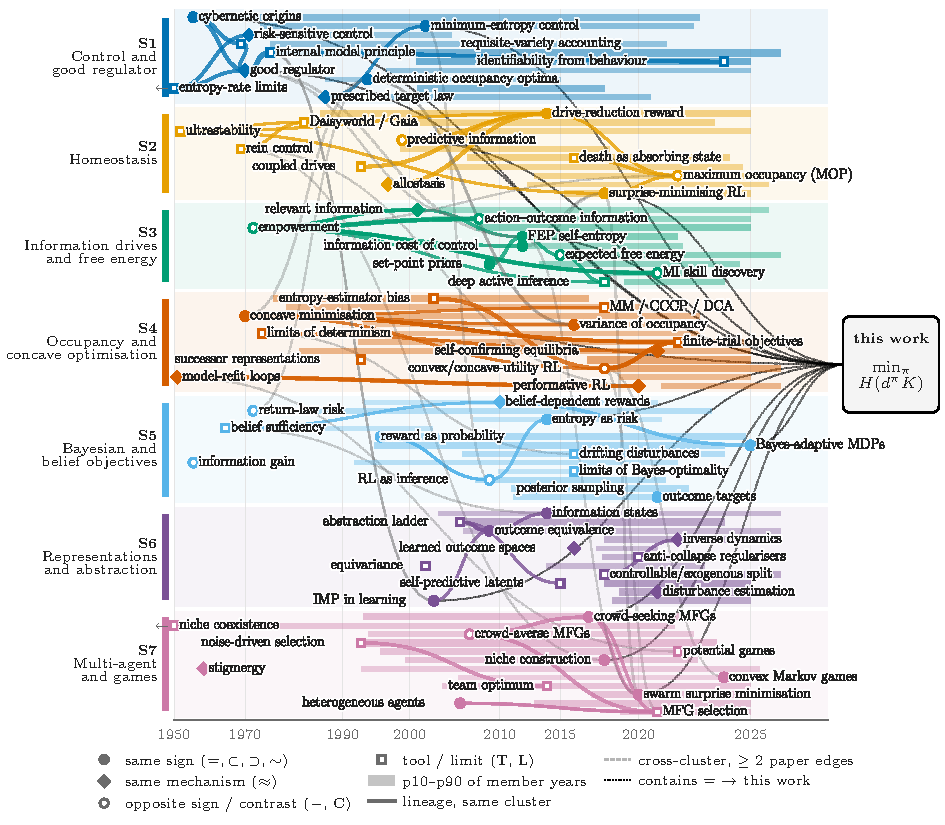
\includegraphics[width=\textwidth]{genealogy_ideas.pdf}
  \caption{Genealogy of the 75 idea nodes of the survey, in seven cluster lanes on a log-past time axis that widens recent decades. Each bar spans the 10th to 90th percentile of its members' publication years, its thickness and opacity grow with member count, and its marker shows the node's relation to our objective, taken from the first code when merged nodes carry several. Edge width is proportional to the number of paper-level lineage edges between two nodes; within a cluster an edge needs two paper edges or one touching a core paper, across clusters it needs two paper edges, and dotted lines join every node coded as sharing our objective to this work. Edges join each idea's first core paper, or its first paper when it has no core paper, so they show which ideas are linked, not when the link was made. Figure~\ref{fig:genealogy} shows the same genealogy paper by paper.}
  \label{fig:ideas}
\end{figure}

\begin{figure}[p]
  \centering
  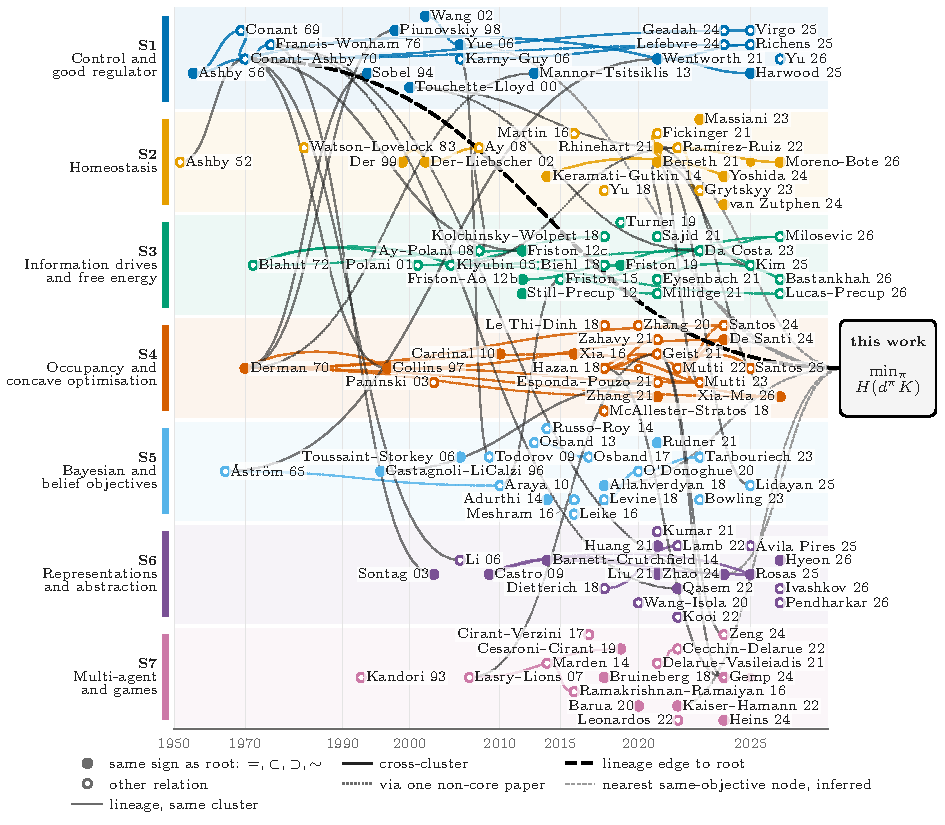
\includegraphics[width=\textwidth]{genealogy.pdf}
  \caption{Genealogy of the 129 core papers in the consolidated survey tree,
    2,456 papers. Each lane is one cluster and each dot is a core paper placed
    at its year on a time axis from 1950 that is close to linear after 2010 and compressed logarithmically before, with position $-\ln(2034.4-\text{year})$. A filled dot marks a paper
    whose node has the same sign as the root objective, and a hollow dot marks
    any other relation. Coloured curves are lineage edges inside a cluster,
    dark curves cross clusters, and dotted curves pass through one non-core
    paper. A thin grey line joins a label to its dot where the label had to
    move. The bold dashed curve is the one lineage edge to the root in the
    data, from Conant and Ashby, while the thin grey dashed curves are inferred
    and only point from the latest core paper of each cluster whose node is
    coded same objective. The four unlabelled dots are papers from 2020 on, and
    all of them are labelled in
    Figure~\ref{fig:genealogy-split}.}
  \label{fig:genealogy}
\end{figure}
\clearpage
\begin{figure}[!t]
  \centering
  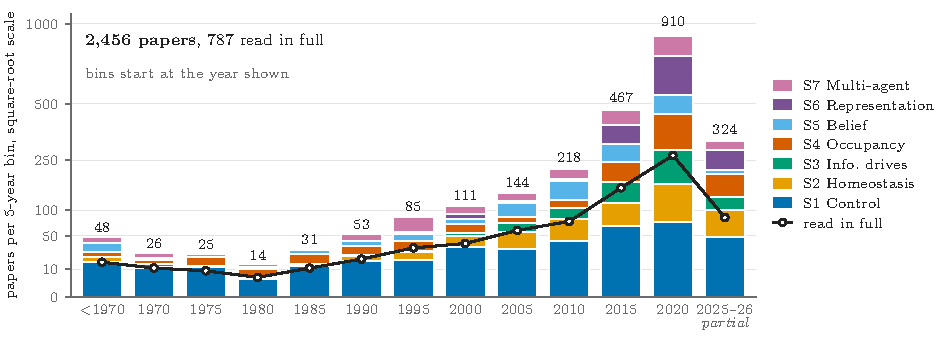
\includegraphics[width=0.9\textwidth]{volume.pdf}
  \caption{Volume of the consolidated survey tree, 2,456 papers, of which 787
    were read in full. Bars count papers per five-year bin, stacked by
    cluster, and the line counts the papers read in full in each bin. The vertical axis is on a square-root scale so that the early bins stay visible; totals and the line remain comparable across bins, but segments higher in a stack look shorter than they are. The last
    bin covers only 2025 and 2026, so its drop reflects coverage rather than
    interest. Most of the literature is recent, and the read-in-full share
    stays near one third until it falls to a quarter in the newest bins.}
  \label{fig:volume}

  \vspace{1.5em}

  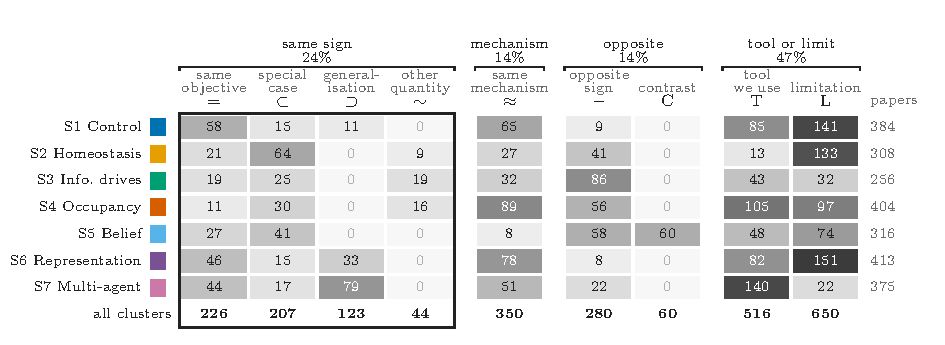
\includegraphics[width=0.9\textwidth]{relation.pdf}
  \caption{Relation of each cluster to the root objective, from the
    consolidated survey tree, 2,456 papers. A cell counts papers, because each
    relation code is assigned to a node and inherited by every member of that
    node, background papers included, so paper counts show how much literature
    sits under each relation while node counts only show how finely a cluster
    was split. Same objective means that the node's stated objective matches
    the minimisation of $H(Z)$ in some form, often static or open-loop, and not
    that its 226 papers already minimise the entropy of the closed-loop outcome
    law over occupancy, which this survey did not find. The outlined block holds
    the four same-sign codes, 24\% of papers, against 14\% of opposite sign or
    contrast and 47\% that supply a tool or a limitation.}
  \label{fig:relation}
\end{figure}

\bibliographystyle{plainnat}
\IfFileExists{notes_joery/joery_survey.bib}
  {\newcommand{\surveybib}{notes_joery/joery_survey}}
  {\newcommand{\surveybib}{joery_survey}}
\bibliography{\surveybib}

\clearpage
\appendix
\section{Genealogy in detail}

Figure~\ref{fig:genealogy-split} splits the genealogy of
Figure~\ref{fig:genealogy} into a backbone over the whole history and a
labelled view of every core paper since 2005.

\begin{figure}[p]
  \centering
  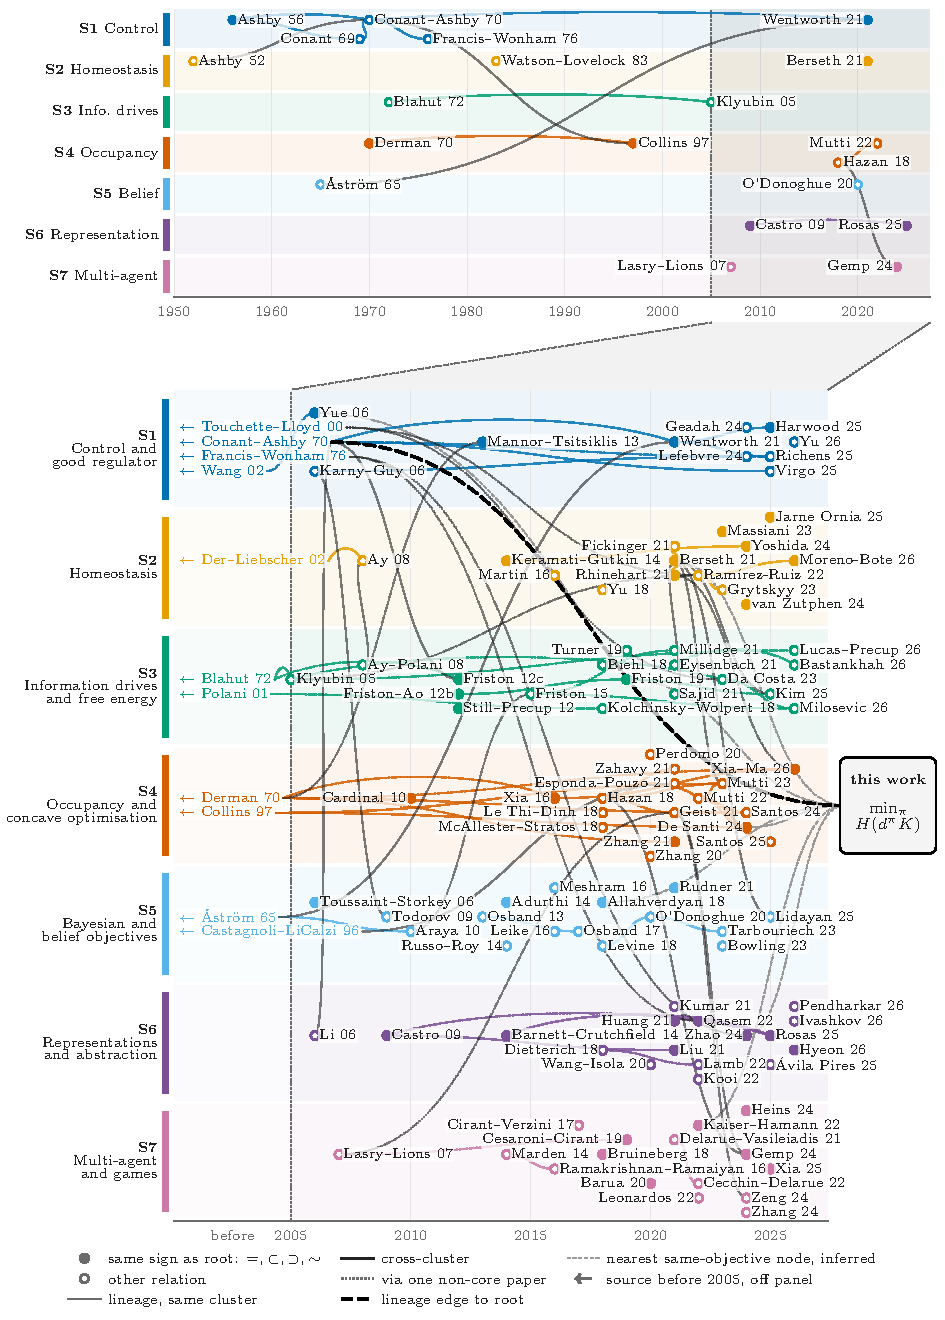
\includegraphics[width=\textwidth,height=0.8\textheight,keepaspectratio]{genealogy_split.pdf}
  \caption{Genealogy of the core papers in two panels, with the markers and
    curves of Figure~\ref{fig:genealogy}. The top panel shows a backbone of 20
    papers on a linear axis from 1950, namely the nine core papers before 1990
    and the most-connected core papers with at least two per cluster, joined
    by the lineage edges among them. The bottom panel zooms into the shaded window from 2005 and
    labels all 108 core papers published since then. Lineage edges from the 11
    earlier papers enter from the left column, where an arrow names the
    source.}
  \label{fig:genealogy-split}
\end{figure}

\end{document}
